\section{SilverTorch Overview}
\label{sec:3}

We propose SilverTorch, a model-based approach to unify recommendation. Instead of building standalone indexing systems, SilverTorch defines all serving components as model layers. The retrieval flow is no different from a forward function execution of tensor operators. Figure \ref{fig:st_arch} illustrates the overall workflow.

After training, a publish flow is executed to compose a SilverTorch model. We initially load trained models. The embedding evaluator utilizes both item features to calculate the item embeddings. We leverage GPUs to calculate the item embeddings. The item embeddings are then processed by the ANN index builder. It quantizes the embeddings to Int8 precision and adopts KMeans++-based~\cite{arthur2006k} training on GPUs. For feature filtering, SilverTorch introduces a novel signature-based GPU index(referred as Bloom Index). The bloom index transforms search index matching to bit operations. Both the ANN index and bloom index are represented as GPU tensors that serve as parameters of the served model.
Meanwhile, User Tower, OverArch layers, and Value Model are quantized to BFloat16 and constructed as model parameters by corresponding builders. The model composer combines all the components into a SilverTorch model. Finally, the model optimizer compiles the eager-mode SilverTorch model into a graph and applies lowering and scripting.
The output from publish is a model snapshot containing all weights tensors and index tensors that can be served in a pure C++ runtime(referred to as predictor).

During online serving,  the predictor runtime is simplified as a forward function execution of a SilverTorch model. 
The SilverTorch retrieval model extracts user features and the filtering query from recommendation request, executes a sequence of kernel operators on GPUs. First, the User Tower computes the user embedding. Subsequently, the Bloom index layer further filters out irrelevant items and generate a mask tensor. The user embedding and the mask tensor are then fed into model's ANN layer and get O(10,000) item ids as pre-filter results. The OverArch layer fetches corresponding item embeddings from embedding cache, and re-rank items by calculating scores and aggregate using the value model across multi-tasks. Final retrieval result returns O(1,000) ids. Final retrieval results are sent to ranking models. 
\begin{figure*}[h]
    \centering
    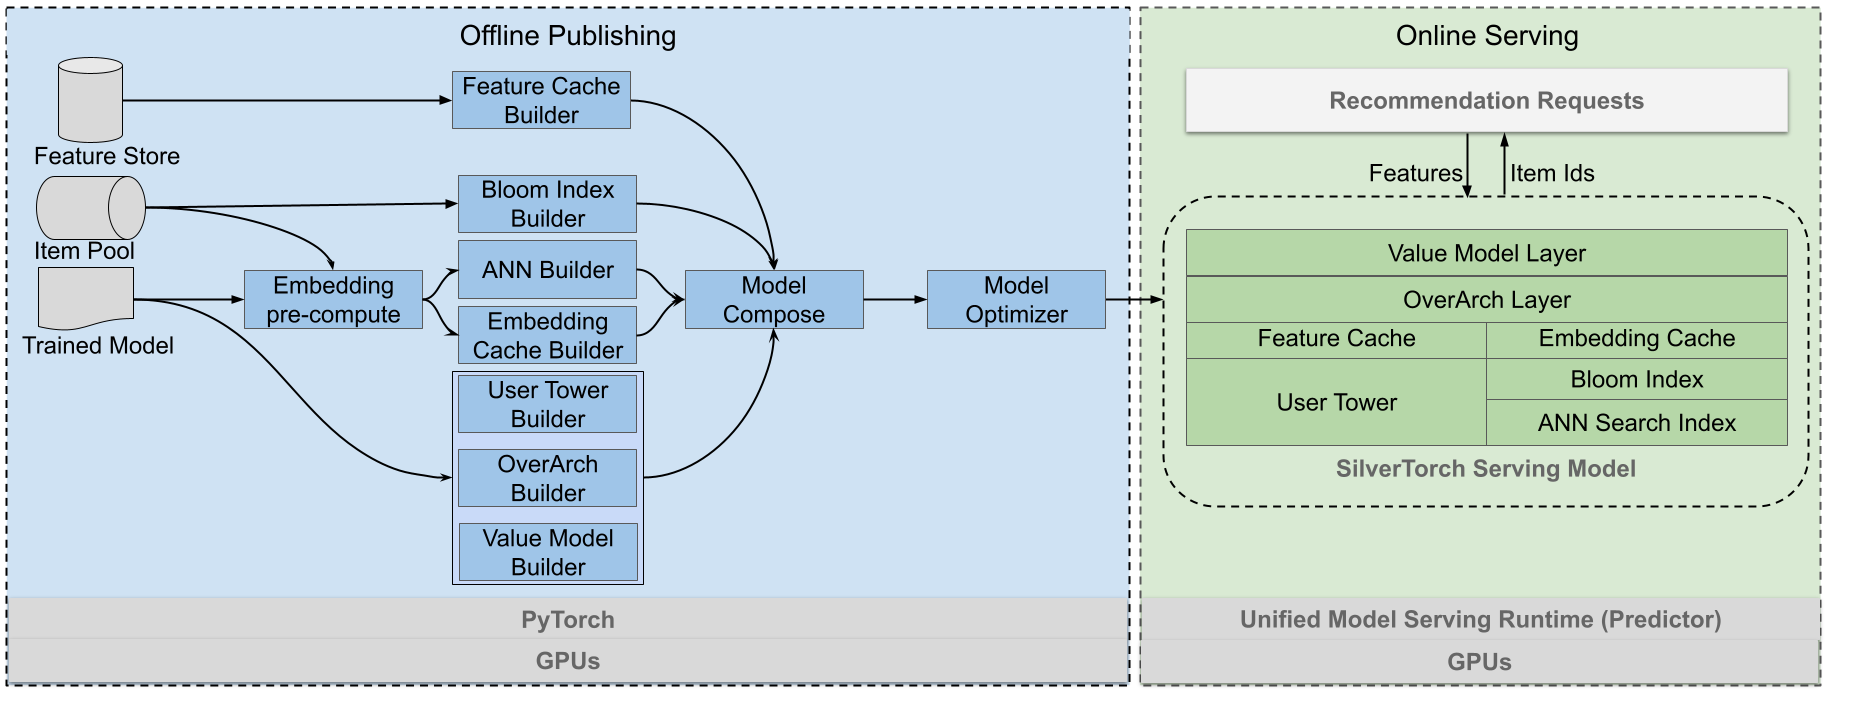
\includegraphics[width=0.8\textwidth]{figures/overview/st_overall.png}
    \caption{Overall workflow of SilverTorch model publish and serving flow.}
    \label{fig:st_arch}
\end{figure*}